\documentclass[a4paper]{article}
\usepackage[utf8]{inputenc}
\usepackage[russian]{babel}
\usepackage[T2]{fontenc}
\usepackage[warn]{mathtext}
\usepackage{graphicx}
\usepackage{floatflt}
\usepackage[left=30mm, top=20mm, right=20mm, bottom=20mm, footskip=10mm]{geometry}


\graphicspath{ {images/} }
\usepackage{multicol}
\setlength{\columnsep}{2cm}


\begin{document}

\begin{titlepage}
	\centering
	\vspace{5cm}
	{\scshape\LARGE Московский физико-технический институт \par}
	\vspace{4cm}
	{\scshape\Large Лабораторная работа \par}
	\vspace{1cm}
	{\huge\bfseries Электромагнитные волны в волноводах \par}
	\vspace{1cm}
	\vfill
\begin{flushright}
	{\large выполнила студентка 653 группы ФФКЭ}\par
	\vspace{0.3cm}
	{\LARGE Карпова Татьяна}
\end{flushright}
	

	\vfill

% Bottom of the page
	Долгопрудный, 2017 г.
\end{titlepage}

\section{Цель работы}
Ознакомление с методами получения и анализа электромагнитных волн СВЧ - диапазона

\section{В работе используются:}
\begin{itemize}
    \item генератор СВЧ типа Г4-83
    \item измерительная линия Р1-28
    \item усилитель 28 ИМ
    \item заглушка
    \item отрезок волновода с поглощающей нагрузкой
    \item отрезки волноводов различных сечений
    \item детекторная головка
\end{itemize}

\section{Теоретические положения}

В СВЧ-диапазоне энергия передаётся с помощью металлических труб,
называемых волноводами (в миллиметровом диапазоне длин волн волноводы могут быть сделаны и из диэлектрика). Электромагнитные волны могут распространяться по металлическим трубам любого профиля, но из технологических соображений сечения волноводов делаются либо
круглыми, либо прямоугольными. \par
Построим э.м. поле в волноводе, складывая падающую и отражённые от стенок плоские волны. Такой метод называется \textit{концепцией Бриллюэна}. \par

\begin{floatingfigure}{41mm}
\noindent
\hfil
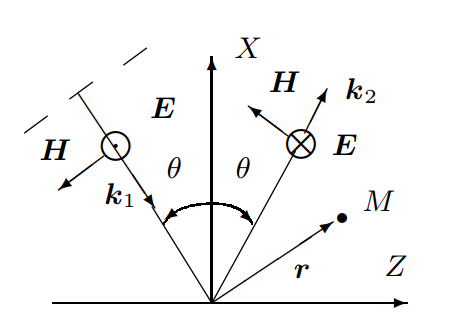
\includegraphics[width=41mm]{fig1.PNG}
\hfil
\caption{Отражение плоской волны от проводящей плоскости}
\label{figCurvesFF}
\end{floatingfigure}

Абсолютное значение волнового вектора \textbf{k} - волновое число - равно
\begin{equation}
k = \frac{2\pi}{\lambda} = \frac{\omega}{v_p_h}
\end{equation}


Уравнения падающей и отражённой электромагнитных волн:
\begin{equation}
    E_1 = E_0 e^{i(\omega t - k_1r)}
\end{equation}

\begin{equation}
    E_1 = - E_0 e^{i(\omega t - k_2r)},
\end{equation}
 где $k_1 = k_2 = \frac{\omega}{c}$. Проекции волновых векторов на оси координат:
 \begin{equation}
     k_1_x = -k cos\theta,\hspace{1cm}   
     k_2_x = k cos\theta,\hspace{1cm}
     k_1_z = k sin\theta,\hspace{1cm} 
     k_2_z = k cos\theta, 
 \end{equation}
 
 Cуммарное электрическое поле в точке М:
 \begin{equation}
     E = E_0[ e^{i(\omega t - k_1r)} - e^{i(\omega t - k_2r)}]
 \end{equation}
 
 Подставляя в (5) координаты вектора $\textbf{r}(x, 0, z)$ и значения $ \textbf{k1} $ и $ \textbf{k2} $ из (4), 
 
 \begin{equation}
     E = 2iE_0 sin(kxcos\theta) e^{i\omega(t - z sin\theta / c)}
 \end{equation}
 
 Это выражение описывает волну с амплитудой
 
 \begin{equation}
     2iE_0 sin(kxcos\theta),
 \end{equation}
 бегущую в направлении $z$ с фазовой скоростью
 
 \begin{equation}
     v_p_h = \frac{c}{sin \theta}
 \end{equation}
 
 Отметим две важные особенности этой волны: 1) её фазовая скорость
больше скорости света; 2) при фиксированном угле θ амплитуда поля
гармонически зависит от $x$ и не меняется со временем. Иначе говоря, в
результате интерференции падающей и отражённой волн в пространстве
над проводящей поверхностью в направлении оси X образуется система стоячих волн. Электрическое поле стоячей волны равно нулю в точках, где $kx cos\theta = n\pi$, т.е. там, где
\begin{equation}
    x = \frac{n \pi}{k cos \theta}
\end{equation}

Мы показали, что в волноводе прямоугольного сечения может распространяться э.м. волна, которую в пределах волновода можно рассматривать как результат суперпозиции двух плоских волн. Каждая плоская волна является чисто поперечной, так что электрическое
и магнитное поля перпендикулярны к направлению их распространения.
В суммарной волне электрическое поле имеет только составляющую $E_y$
и, следовательно, перпендикулярно оси волновода, а магнитное поле имеет составляющие $H_x$ и $H_z$ \par

\textit{Электромагнитное поле в волноводе не является чисто поперечным, а имеет продольные составляющие.}

Если даны две параллельные проводящие плоскости, расположенные на расстоянии $a$ друг от друга, то между ними могут распространяться волны, если

\begin{equation}
    cos \theta_n = \frac{n\pi}{ka} = \frac{n\lambda_0}{2a} = \frac{n\pic}{a\omega},
\end{equation}
где $\lambda_0$ -- длина волны в свободном пространстве. \par

Движение э.м. волны по волноводу возможно, если углы падения подчиняются условию

\begin{equation}
     cos \theta_n = \frac {n\lambda_0}{2a} \le 1
\end{equation}

Нижняя критическая частота волны
\begin{equation}
    \omega_c_r = \frac{\pi c}{a}
\end{equation}

и верхняя критическая длина волны
\begin{equation}
    \lambda_c_r = 2a
\end{equation}

соответствуют $n = 1$ \par

Выражение для фазовой скорости э.м. волны, распространяющейся в волноводе:

\begin{equation}
    v_p_h = \frac{c}{\sin \theta} = \frac{c}{\sqrt{1 - \cos^2\theta}} = \frac{c}{\sqrt{1 - (\omega_c_r/\omega)^2}}
\end{equation}

Фазовая скорость (скорость перемещения поверхности постоянной фазы $v+p+h = \omega / k$) в волноводе больше скорости света в пустоте, а групповая (скорость распространения возмущения $u = d\omega / dk$) всегда меньше.

Волновое число $k_z$, описывающее распространение волны вдоль волновода:

\begin{equation}
    k_z = \frac{\omega}{v_p_h} = \frac{\omega}{c}\sqrt{1 - (\frac{\omega_c_r}{\omega})^2}
\end{equation}

При частотах $\omega < \omega_c_r = \pi c/a$ волны вдоль трубы экспоненциально затухают. Поэтому критическую частоту называют граничной частотой волновода.

Преобразуя соотношение (15), можно связать длины волн в волноводе ($\lambda_w$), в открытом пространстве ($\lambda_0$) и критическую ($\lambda_c_r$):

\begin{equation}
    \frac{1}{\lambda_w^2} = \frac{1}{\lambda_0^2} - \frac{1}{\lambda_c_r^2}
\end{equation}

В случае прямоугольного волновода с поперечными размерами $a$ и $b$ все возможные критические длины волн определяются общей формулой

\begin{center}
    $\lambda_c_r = \frac{1}{\sqrt{(\frac{m}{2a})^2 + (\frac{n}{2b})^2}}$
\end{center}

Величина $m$ представляет собой полное число полупериодов изменения той или иной составляющей поля вдоль пути, идущего параллельно широкой стенке волновода ($a$), а $n$ — то же для узкой стенки ($b$). \par

Если в волноводе имеется какое-либо препятствие, нерегулярность (в предельном случае он просто закрыт металлической пластиной), то в нём появляется отражённая волна. Падающая и отражённая волны интерферируют
и создают в волноводе стоячую волну. Прямая волна, движущаяся в положительном направлении оси Z:

\begin{center}
    $E_1 = E_0 e^{i(\omega t - k_z z)}$,
\end{center}
а отражённая - 
\begin{equation}
    E_2 = \rho E_0 e^{i(\omega t + k_z z + \phi)},
\end{equation}

где $\rho$ — коэффициент отражения по амплитуде, а $\phi$ — фаза отражённой волны. Суммарное поле в волноводе имеет вид

\begin{center}
    E(z) = E_1 + E_2 = E_0 e^{-ik_z z}(1 + \rho e^{i(2k_z z + \phi)}e^{i\omega t}) = A_0 e^{i\omega t}
\end{center}

Из этого выражения видно, что в каждом сечении волновода (z = const)
поле зависит от времени по гармоническому закону, а квадрат амплитуды
равен

\begin{equation}
    A_0^2 = E_0^2[1 + \rho^2 + 2\rho \cos(2k_z z + \phi)]
\end{equation}

Максимальное (в пучности) и минимальное (в узле) значения поля
равны соответственно:

\begin{equation}
    E_m_a_x = E_0 (1 + \rho), \hspace{1cm} E_min = E_0 (1 - \rho)
\end{equation}

Из формулы (18) следует, что расстояние l между соседними узлами (или
пучностями) составляет

\begin{equation}
    l = \frac{\pi}{k_z} = \frac{\lambda_w}{2}
\end{equation}

Это даёт удобный способ измерения длины волны λв в волноводе.
Отношение

\begin{equation}
    K = \frac{E_m_a_x}{E_m_i_n}
\end{equation}

называется коэффициентом стоячей волны (к.с.в.). Из (19) следует, что
коэффициент отражения от препятствия по амплитуде

\begin{equation}
    \rho = \frac{E_m_a_x - E_m_i_n}{E_m_a_x + E_m_i_n} = \frac{K - 1}{K + 1}
\end{equation}

В случае полного отражения (металлическая заглушка) $\rho$ = 1, а если
в волновод вставлено вещество, поглощающее СВЧ-излучение (согласованная нагрузка), то $\rho$ = 0.

\section{Экспериментальная установка}
\subsection{Волны в волноводе при частоте выше критической}

\begin{figure}[h]
    \centering
    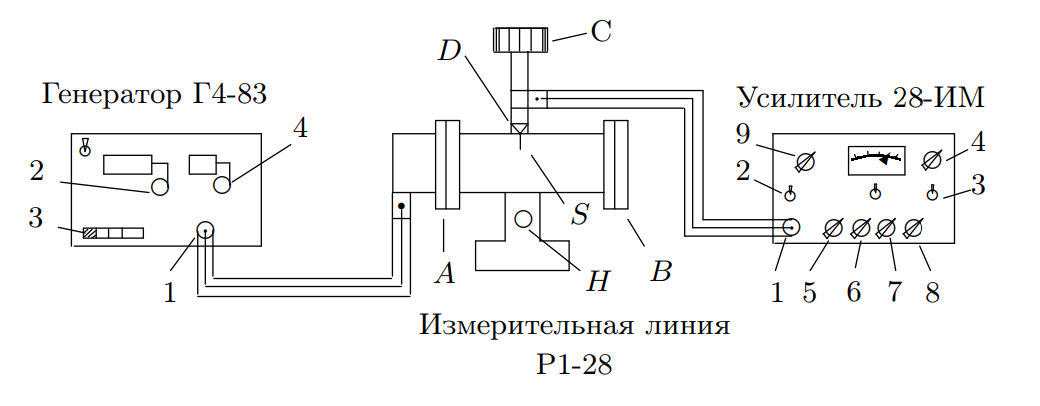
\includegraphics[width=\textwidth]{fig2.PNG}
    \caption{Схема для исследования структуры волн СВЧ}
    \label{fig:vac}
\end{figure}

Схема для исследования структуры волн в волноводе при частоте выше критической представлена на рис. 2. Модулированный сигнал от высокочастотного генератора (цуги с частотой повторения 1 кГц) поступает на вход A измерительной линии, вдоль которой перемешается зонд S. Высокочастотный сигнал с зонда поступает на кристаллический детектор D. \par

С нагрузки детектора (c RC-цепочки) снимается огибающая высокочастотного сигнала и подаётся на усилитель низкой частоты. Величина сигнала регистрируется вольтметром, вмонтированным в усилитель. Ручка C — настройка измерительной линии — служит для согласования зонда (как антенны) со входом усилителя.
В волноводе с закрытым выходом образуется стоячая волна. Определив расстояние между узлами, можно рассчитать длину волны
и фазовую скорость СВЧ-сигнала в волноводе. Устройство детекторной головки, установленной на измерительной линии, таково, что отклик вольтметра U на величину напряжённости электрического поля E в волноводе пропорционален $E^n$
\begin{equation}
    U \propto E^n,
\end{equation}
а показатель степени n сам зависит от величины сигнала: при малых
сигналах детектирование квадратичное ($n = 2$), при больших — линейное ($n = 1$). Если известно распределение поля $E(z)$ вдоль измерительной линии, то, изучив распределение $U(z)$, можно по графику $ln(U) = f[ln(E)]$ определить характер детектирования: в двойном логарифмическом масштабе любая степенная функция — прямая линия, по наклону которой можно определить $n$. Распределение $E(z)$ нетрудно рассчитать для волновода с закороченным концом (металлической заглушкой), когда фаза отражённой волны $\phi = \pi$, а $\rho = 1$. Как следует из (17), электрическое поле в этом случае имеет вид:

\begin{equation}
    E(z) = E_0 e^{-ik_1 z}(1 - e^{2ik_z z})e^{i\omega t} = E_0 e^{i\omega t}(e^{-ik_1 z} - e^{ik_1 z}) = 2E_0 e^{i\omega t} sin(k_z z) \propto sin(k_z z),
\end{equation}
где $z$ -- смещение от узла. \par
Меняя нагрузку на выходе измерительной линии (B на рис. 2) и сравнивая максимальное и минимальное показания вольтметра, можно рассчитать
коэффициент стоячей волны (к.с.в.) и коэффициент отражения $\rho$.

\subsection{Волны в волноводе при частоте ниже критической}

\begin{figure}[h]
    \centering
    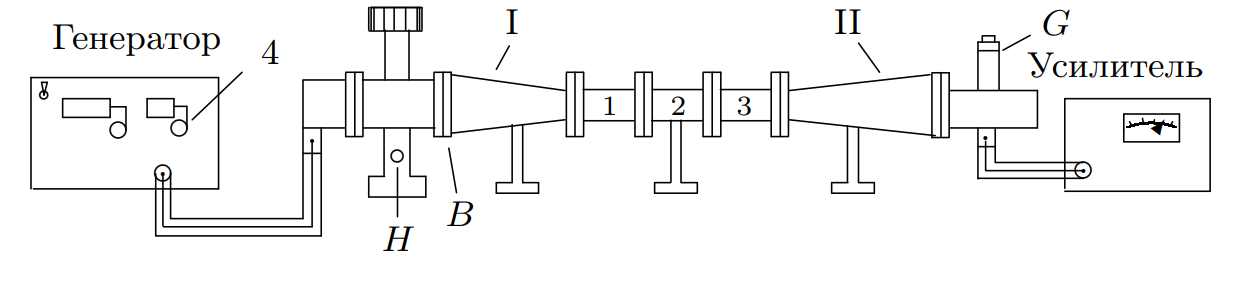
\includegraphics[width=\textwidth]{fig3.PNG}
    \caption{Схема для исследования затухания}
    \label{fig:vac}
\end{figure}

Для исследования затухания волн в волноводе при частоте ниже кри-
тической используются те же генератор, усилитель, измерительная линия
и дополнительный набор волноводов с отдельной детекторной головкой G (рис. 3). Дополнительный набор начинается и заканчивается волноводами переменного сечения I и II. Между ними можно разместить 1, 2 или 3 одинаковых отрезка с постоянным сечением. В такой системе волны
с частотами меньше критической экспоненциально затухают. \par
Мощность сигнала на выходе из волновода $W$ можно связать с мощностью входного сигнала $W_0$ двумя способами:

\begin{center}
    $W = W_0 e^{-\alpha z}$ или $ W = W_0 10^{-\beta z}$, z -- длина волновода.
\end{center}
 Коэффициент ($\alpha z$) измеряется в неперах (Нп). 1 непер соответствует отношению интенсивностей, равному основанию натуральных логарифмов. Коэффициент ($\beta z$) принято измерять в децибелах [дБ]: один бел соответствует уменьшению мощности в 10 раз; децибел — одна десятая бела. Измеренное в децибелах затухание определяется формулой

\begin{center}
   $ (\beta z) = 10 lg\frac{W_0}{W}$
\end{center}

Из этого определения вытекает, что

\begin{equation}
    \alpha = 2,3 \beta
\end{equation}

Как следует из (17), в закритическом волноводе при квадратичном детектировании интенсивность сигнала падает по закону $E^2 \propto e^{-\alpha z}$, где α — коэффициент затухания:

\begin{center}
    $\alpha = 2ik_z$
\end{center}

Подставляя волновое число из (15) и заменяя частоты с помощью (10) и (12), найдём

\begin{equation}
    \alpha = 2ik_z = \frac{2\omega}{c} \sqrt{(\frac{\omega_c_r}{\omega})^2 - 1} = \frac{2\pi}{a}\sqrt{1 - (\frac{2a}{\lambda_0})^2}
\end{equation}

Здесь $\lambda_0 = c/\nu = 3,22$ см — длина волны в свободном пространстве, соответствующая рабочей частоте $\nu = 9320$ МГц, $a = 1,6$ см — размер
широкой стенки волновода-вставки.

\section{Выполнение работы}
\subsection{Исследование структуры волн при частоте выше критической}
\begin{enumerate}
\subsubsection{Определение длины волны СВЧ-сигнала в волноводе}
    \item Определим критическую частоту для данного волновода по формуле $\nu_c_r = c/2a = 6517$ МГц ($a = 23$ мм), она больше рабочей частоты $9320$ МГц. Проведём настройку приборов.
    \item Снимем зависимость показаний вольтметра $U$ от положения зонда $z$. Результаты занесём в таблицу 1.
    
    \begin{table}[h]
    \centering
    \begin{center}
    \caption{Показания вольтметра в зависимости от положения зонда на измерительной линии}
    \end{center}
    \vspace{0.1cm}
    \label{tab:my_label}
    \begin{tabular}{ |p{1.5cm}||p{0.5cm}|p{0.5cm}|p{0.5cm}|p{0.5cm}|p{0.5cm}|p{0.5cm}|p{0.5cm}|p{0.5cm}|p{0.5cm}|p{0.5cm}|p{0.5cm}|p{0.5cm}|p{0.5cm}|p{0.5cm}|p{0.5cm}|  }
 \hline
 $U$, мВ & 37 & 25 & 16 & 7,8 & 2,9 & 0,3 & 0,54 & 3,5 & 9,7 & 19 & 29 & 43 & 57 & 72 & 84   \\
\hline 
 $z$, мм & 0 & 1 & 2 & 3 & 4 & 5 & 6 & 7 & 8 & 9 & 10 & 11 & 12 & 13 & 14 \\
 \hline 
 \hline 
 
 $U$, мВ & 91 & 99 & 101 & 98 & 85 & 75 & 62 & 47 & 32 & 22 & 12 & 5,2 & 1,25 & 0,09 & 1,8 \\
 \hline 
  $z$, мм & 15 & 16 & 17 & 18 & 19 & 20 & 21 & 22 & 23 & 24 & 25 & 26 & 27 & 28 & 29  \\
 \hline 
 \hline 
 $U$, мВ & 6,15 & 14 & 23 & 36 & 49.5 & 64 & 78 & 89 & 98 & 102 & 97 & 90 & 78 & 66 & 52 \\  
 \hline
  $z$, мм & 30 & 31 & 32 & 33 & 34 & 35 & 36 & 37 & 38 & 39 & 40 & 41 & 42 & 43 & 44 \\
 \hline
\end{tabular}

\end{table}
    
    \item Построим график $U = f(z)$ (рис. 4) и определим по нему длину волны $\lambda_w$ в волноводе. $\lambda_w = 22$ мм. Используя формулу (16), рассчитаем теоретическое значение длины волны в волноводе: $\lambda_w = (\frac{1}{\lambda_0^2}-\frac{1}{\lambda_c_r^2})^{-1/2} = 44,54$ мм
    
\begin{figure}[h]
    \centering
    \caption{Зависимость показаний вольтметра от положения зонда}
    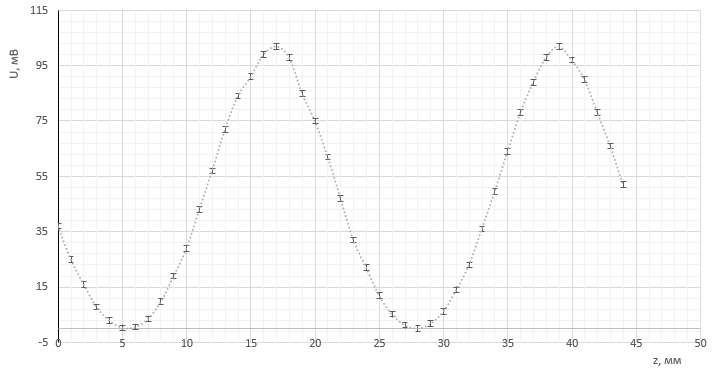
\includegraphics[width=\textwidth]{graph1.PNG}
    \label{fig:vac}
\end{figure}
\end{enumerate}

 \item Расстояние между соседними узлами в стоячей волне составляет 1/2 длины свободной волны. По графику определяем длину свободной волны в волноводе $\lambda_w = 2l = 44,5$ мм. Она совпадает с длиной волны $\lambda_w = 44,54$ мм, рассчитанной теоретически. Отсюда можем судить, что в данном режиме работы зонд исправен и даёт точные показания. \par
 Длина волны в свободном пространстве $\lambda_0 = 32,2$ мм меньше критической длины волны $\lambda_c_r = 46$ мм. \par 
 Фазовая скорость волн в волноводе из (14) $v_p_h = \frac{c}{\sqrt{1 - (\omega_c_r/\omega)^2}} = \frac{c}{\sqrt{1 - (\nu_c_r/\nu)^2}} = 419361,71$ км/с, $v_p_h > c$. Это не противоречит законам, так как с такой скоростью перемещаются узлы волн, при этом не передаётся ни энергия, ни информация (именно они не могут передаваться со скоростью, большей скорости света в вакууме).  \par
 Групповая скорость $u = \frac{c^2}{v_p_h} = 214315,04$ км/с.
\subsubsection{Определение характера детектирования}
\begin{enumerate}
    \item Перемещая зонд вблизи узла 28 мм, оценим диапазон измерений вольтметра U. Снимем зависимость $U$ от координаты зонда вблизи узла ($z = \pm 1$ мм), фиксируя значения множителей $K_5$ и $K_9$. Результаты занесём в таблицу 2.
    
    \begin{table}[h]
    \centering
    \begin{center}
    \caption{Изменение показаний вольтметра при перемещении вблизи узла}
    \end{center}
    \vspace{0.1cm}
    \label{tab:my_label}
    \begin{tabular}{ |p{1.5cm}||p{0.5cm}|p{0.5cm}|p{0.5cm}|p{0.5cm}|p{0.5cm}|p{0.5cm}|p{0.5cm}|p{0.5cm}|p{0.5cm}|p{0.5cm}|p{0.5cm}|  }
 \hline
 $U$, мВ & 0,83 & 0,59 & 0,39 & 0,24 & 0,17 & 0,08 & 0,07 & 0,11 & 0,22 & 0,36 & 0,66   \\
\hline 
 $z$, мм & 1 & 0,8 & 0,6 & 0,4 & 0,2 & 0 & 0,2 & 0,4 & 0,6 & 0,8 & 1 \\
 \hline
\end{tabular}
\end{table}
    
    \begin{figure}[h]
    \centering
    \caption{Определение характера детектирования зонда по графикам}
    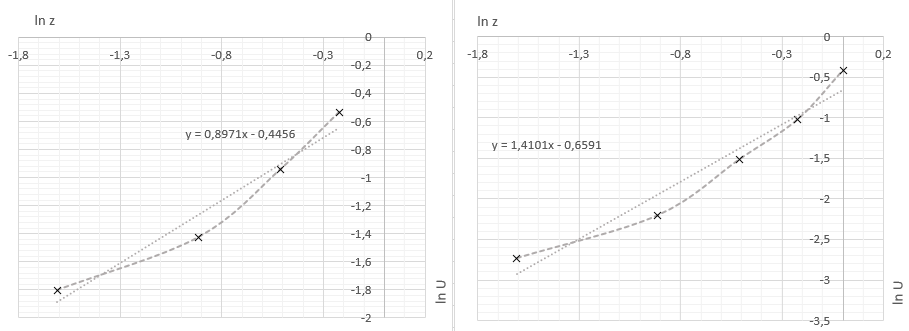
\includegraphics[width=\textwidth]{graph4.PNG}
    \label{fig:vac}
\end{figure}

    \item Аппроксимируя зависимость $ln(U) = f(ln(z))$ к прямой и вычисляя коэффициент наклона аппроксимирующей прямой, определяем характер детектирования зонда. Коэффициент при аргументе примерно равен 1, если принять во внимание оба графика - \textit{характер детектирования в этом эксперименте линейный}
\end{enumerate}

\subsubsection{Определение коэффициентов отражения}
\begin{enumerate}
    \item Снимем металлическую заглушку с фланца измерительной линии, измерим максимальное и минимальное напряжения в волне
    \begin{center}
        $U_m_a_x = 162$ мВ \hspace{2cm} $U_m_i_n = 43$ мВ
    \end{center}
    
    \item Наденем на выходной фланец измерительной линии отрезок волновода с поглощающей нагрузкой, измерим максимальное и минимальное напряжения в волне
    \begin{center}
        $U_m_a_x = 96$ мВ \hspace{2cm} $U_m_i_n = 71$ мВ
    \end{center}
    
    \item По формуле (22) определим коэффициенты отражения от препятствия по амплитуде для открытого, закрытого волновода и для волновода с поглощающей нагрузкой
    \begin{center}
        $\rho_{closed} = 0,998$ \hspace{1cm} $\rho_{opened} = 0,580$ \hspace{1cm} $\rho_{load} = 0,151$
    \end{center}
    
    Только по значениям коэффициентов отражения можно было бы определить состояние волновода. При $\rho \approx 1$ волновод наглухо закрыт металлической заглушкой ($\rho_{closed} = 0,998$), при $\rho \approx 0$ на конце волновода поставлено вещество, поглощающее СВЧ-излучение ($\rho_{load} = 0,151$). Воздух не препятствует распространению СВЧ-волн, но в воздушной среде при распространении излучение становится менее интенсивным ($\rho_{opened} = 0,580$)
    
\end{enumerate}

\subsection{Исследование затухания волн при частоте ниже критической}
\begin{enumerate}
    \item Соберем схему согласно рис. 3, измерим длину каждой секции.
    \begin{center}
        $l_{gold} = 4,95$ см \hspace{0.5cm} $l_{blue} = 3,95$ см \hspace{0.5cm} $l_{white} = 5,7$ см  \\
        $l_{var} = 14,5$ см \hspace{0.5cm} $l_{line} = 15,3$ см \hspace{0.5cm} $l_{det} = 10,1$ см  \\
    \end{center}
    
    Критическая частота для этого эксперимента $\nu_c_r = c/2a = 9368,5$ МГц, рабочая частота $\nu = 9320$ МГц $< \nu_c_r$
    \item Последовательно уменьшая количество секций волновода от трёх до нуля, будем подбирать такое ослабление $\gamma$ с генератора, чтобы показания вольтметра на усилителе ($U = 5$ мВ) оставались неизменными. Результаты занесём в таблицу 3.
    
\begin{table}[h]
    \centering
    \begin{center}
    \caption{Зависимость ослабления от длины волновода}
    \end{center}
    \vspace{0.1cm}
    \label{tab:my_label}
    \begin{tabular}{ |p{1.5cm}||p{0.7cm}|p{0.7cm}|p{0.7cm}|p{0.7cm}|  }
 \hline
 $\gamma$, дБ & 20 &26,2 &28,8 &33,45    \\
\hline 
 $z$, cм & 70 & 66.05 & 60,35 & 55,4  \\
 \hline
\end{tabular}
\end{table}

\item
Построим график зависимости ослабления $\gamma$ от длины волновода $z$ (рис. 6) \par
\begin{figure}[h]
    \centering
    \caption{Зависимость ослабления входящего сигнала от длины волновода}
    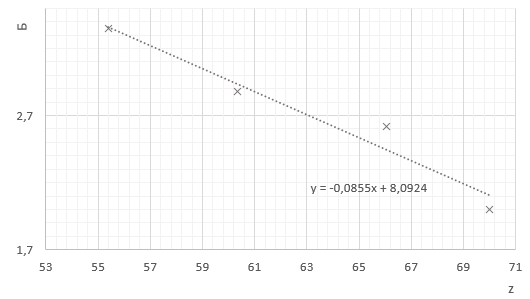
\includegraphics[width=15cm]{graph5.PNG}
    \label{fig:vac}
\end{figure}

По углу наклона графика определим значение коэффициента затухания $\beta$: $\beta = - \gamma/z = 0,0855$ Б/см. Тогда коэффициент $\alpha = 2,3\beta = 0,1969$ Нп/см.\par
Рассчитаем теоретические значения коэффициентов $\alpha$ и $\beta$. Если при квадратичном детектировании интенсивность сигнала падает по закону $E^2 \propto e^{-\alpha z}$, где $\alpha = 2ik_z$, то при линейном детектировании $E \propto e^{\alpha z}$ или $\alpha = ik_z$. Тогда, преобразовав формулу (26) по линейный характер детектирования, получим, что
\begin{center}
    $\alpha = ik_z = \frac{\pi}{a}\sqrt{1 - (\frac{2a}{\lambda_0})^2} = 0,2184$ Нп/см \\
    $\beta = \alpha / 2,3 = 0,0950$ Б/см. 
\end{center}
В итоге, сравнивая теоретические и экспериментальные данные:

\begin{center}
    $\alpha_t_h = 0,218$ Нп/см \hspace{1cm} $\alpha_e_x = 0,197$ Нп/см\\
    $\beta_t_h = 0,095$ Б/см \hspace{1cm} $\beta_e_x = 0,086$ Б/см
\end{center}

Результаты, полученные теоретически и экспериментально, практически совпадают. Примечательно, что если бы мы использовали формулу для квадратичного детектирования, указанную в указании к работе, результаты бы не совпали (см. вывод)

    
\end{enumerate}

\newpage

\section{Вывод}
В ходе работы было исследовано распространение СВЧ-волн в волноводах различных сечений. Проанализированы результаты измерения различных параметров волн при их частоте выше и ниже критической для соответсвующего волновода.
\begin{enumerate}
    \item Была измерена длина волны в волноводе при частоте выше критической. Передвигая зонд, подсоединённый к усилителю с вольметром, измерялась величина СВЧ-сигнала (стоячая волна). Данным методом получилось с большой точностью определить длину волны в волноводе:
    
\begin{center}
    $\lambda_{w(th)} = 44,54$ мм \hspace{2cm} $\lambda_{w(ex)} = 44,50$ мм
\end{center}
    
    Также определена фазовая скорость волны в волноводе
\begin{center}
    $v_p_h = = 419361,71$ км/с
\end{center}
     и её групповая скорость
     \begin{center}
          $u = 214315,04$ км/с.
     \end{center}
     
\item
    Определён характер детектирования зонда при малых сдвигах от местоположения узла волны. Он оказался линейным, а не квадратичным.
    
\item
    Определены коэффициенты отражения волны от разных материалов - металлическая заглушка, воздушное пространство и поглощающая нагрузка.
  \begin{center}
        $\rho_{closed} = 0,998$ \hspace{1cm} $\rho_{opened} = 0,580$ \hspace{1cm} $\rho_{load} = 0,151$
    \end{center}  
    Действительно, в теории коэффициент отражения от металлической заглушки $\approx 1$, от поглощающей нагрузки $\approx 0$

\item
    Было исследовано затухание СВЧ-волн при частоте ниже критической. В этом пункте при выполнении работы были замечены значительные несоответствия теории, предложенной в указании к работе, и экспериментальными данными. 
\begin{itemize}
    \item Во-первых, формула $\gamma = \beta z$ неверна чисто с логической точки зрения. $\beta$ -- коэффициент затухания - по определению $\beta z = 10 lg\frac{W_0}{W}$ должен быть больше нуля (так как при длине волны ниже критической мощность сигнала на входе $W_0$, очевидно, больше мощности на выходе $W$). С другой стороны, при \textit{уменьшении} длины волновода для того, чтобы сигнал на выходе оставался тем же, нужно \textit{ослаблять} входящий сигнал, то есть увеличивать ослабление. Таким образом, при уменьшении $z$ должна увеличиваться $\gamma$, но при $\beta > 0$ и $\gamma = \beta z$ это не выполняется. Получается, нужная нам формула
\begin{center}
      \fbox{$\gamma = -\beta z$}.  
\end{center}

    
    \item
    Во-вторых, в описании к работе указаны формулы, принимая, что детектирование зонда квадратичное. Учитывая результаты измерений п. 5.1.2, мы вывели формулу для линейного характера детектирования и получили значения коэффициентов затухания $\alpha$ и $\beta$, очень близкие к практическим. Теперь посчитаем теоретические значения этих коэффициентов для квадратичного детектирования.
    
\begin{center}
    $\alpha = 2ik_z = \frac{2\pi}{a}\sqrt{1 - (\frac{2a}{\lambda_0})^2} = 0,4368$ Нп/см \\
    $\beta = \alpha / 2,3 = 0,1899$ Б/см. 
\end{center}
    Эти значения почти в 2 раза больше, чем полученные экспериментально $\alpha = 2,3\beta = 0,1969$ Нп/см и $\beta = - \gamma/z = 0,0855$ Б/см.
    
    Полученная нами формула $\alpha = ik_z$ гораздо лучше описывает практические результаты
    
\begin{center}
    $\alpha_t_h = 0,218$ Нп/см \hspace{1cm} $\alpha_e_x = 0,197$ Нп/см\\
    $\beta_t_h = 0,095$ Б/см \hspace{1cm} $\beta_e_x = 0,086$ Б/см
\end{center}
    
\end{itemize}
    
\end{enumerate}


\end{document}
